\documentclass{article}
\usepackage{tikz}

\begin{document}

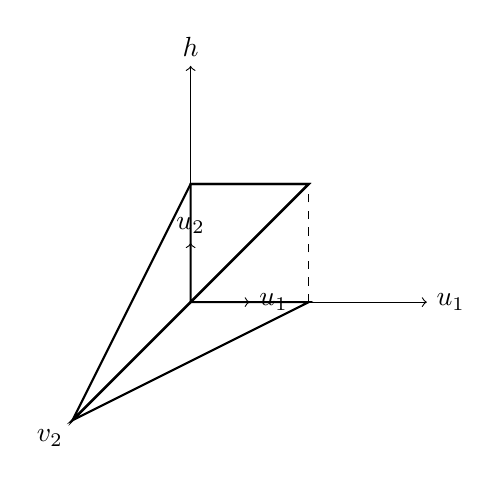
\begin{tikzpicture}[scale=1.5]
    % Define coordinates
    \coordinate (A) at (-1,-1);
    \coordinate (B) at (0,0);
    \coordinate (C) at (1,0);
    \coordinate (D) at (0,1);
    \coordinate (E) at (1,1);
    
    % Draw the polytope
    \draw[thick] (A) -- (B) -- (C) -- cycle;
    \draw[thick] (B) -- (D) -- (E) -- cycle;
    \draw[thick] (A) -- (D) -- (E) -- cycle;
    
    % Draw dashed lines
    \draw[dashed] (B) -- (D);
    \draw[dashed] (C) -- (E);
    \draw[dashed] (A) -- (D);
    
    % Draw axes
    \draw[->] (0,0) -- (2,0) node[right] {$u_1$};
    \draw[->] (0,0) -- (0,2) node[above] {$h$};
    
    % Label vertices
    \node at (A) [below left] {$v_2$};
    \node at (B) [below right] {};
    \node at (C) [above right] {};
    \node at (D) [above left] {};
    \node at (E) [above right] {};
    
    % Draw arrows for u1 and u2
    \draw[->] (B) -- ++(0.5,0) node[right] {$u_1$};
    \draw[->] (B) -- ++(0,0.5) node[above] {$u_2$};
\end{tikzpicture}

\caption{The polytope \( P_1 \) corresponding to \( \mathbb{P}^2 \) with \( v_1 = (1,0) \), \( v_2 = (0,1) \), \( v_3 = (-1,-1) \).}
\end{document}